%!TEX program = xelatex
%!BIB program = bibtex

\documentclass[cn,black,9pt,normal]{elegantnote}
\usepackage{float}
\usepackage{hyperref}

\newcommand{\upcite}[1]{\textsuperscript{\textsuperscript{\cite{#1}}}}

\title{数码摄影作业(01)摄影历史上的第一次\\\small{第一个CMOS感光元件拍摄的照片}}
\author{姓名:姜文渊\\学号:1951510}
%\institute{School of Life Science, Tongji University}
%\version{1.00}
\date{2021年3月11日}

\begin{document}

\maketitle


\section{CMOS感光元件简介}

CMOS图像传感器是一种典型的固体成像传感器,与CCD有着共同的历史渊源。
相比于价格昂贵的CCD传感器,CMOS价格相对低廉(良品率高,集成度高),被广泛运用于各类中低端摄影器材中。
由于CMOS传感器的每个象素由四个晶体管与一个感光二极管构成(含放大器与A/D转换电路),
使得每个象素的感光区域远小于象素本身的表面积,因此在象素尺寸相同的情况下,CMOS传感器的灵敏度要低于CCD传感器。
此外,CMOS传感器的每个象素都比CCD传感器复杂,其象素尺寸很难达到CCD传感器的水平。
CMOS的这些小缺点逐渐随着半导体工业的制程进步而被改良,以至于直至今日,
摄影爱好者入门的第一个设备大多使用的是CMOS感光元件,
而曾经主流的CCD元件则逐渐脱离主流市场。\upcite{fossum1993active}

笔者的第一只相机,\texttt{佳能M200}采用的即是2410万像素CMOS。

\section{第一个CMOS感光元件}

CMOS Image Sensor (CIS) 最早是美国喷气推进实验室(Jet Propulsion Laboratory, JPL)的一个研究项目,Dr. Eric Fossum 是业界公认的CIS技术发明人。

1992年,Dr. Eric R. Fossum 在美国加州Pasadena(帕萨迪纳)的喷气推进实验室工作,负责NASA一些雄心勃勃的太空探测器的建造和运行。
那一年NASA向员工们发出了一个颇为有趣的要求 ——“更快,更好,更便宜”。作为JPL图像传感器研究的负责人,
Fossum 负责重新发明NASA太空船上的巨型相机。当时在数码摄影市场上已经应用了CCD技术,但是CCD需要消耗大量的能量和相当多的支持芯片。
Fossum 团队发现,如果能够消除在成像阵列中反复转移电荷的需要,那么这两个问题都将解决,于是就诞生了CMOS有源像素传感器。\upcite{LL2020}
下图是JPL 首个CMOS APS 芯片和其拍摄的照片,只有28x28个像素(对比现在的上亿像素的CMOS元件),像素尺寸40umx40um,诞生于1993年4月。\upcite{fossum2020invention}(APS 是Active Pixel Sensor (主动像素传感器)的缩写。)
\begin{figure}[h]
    \centering
    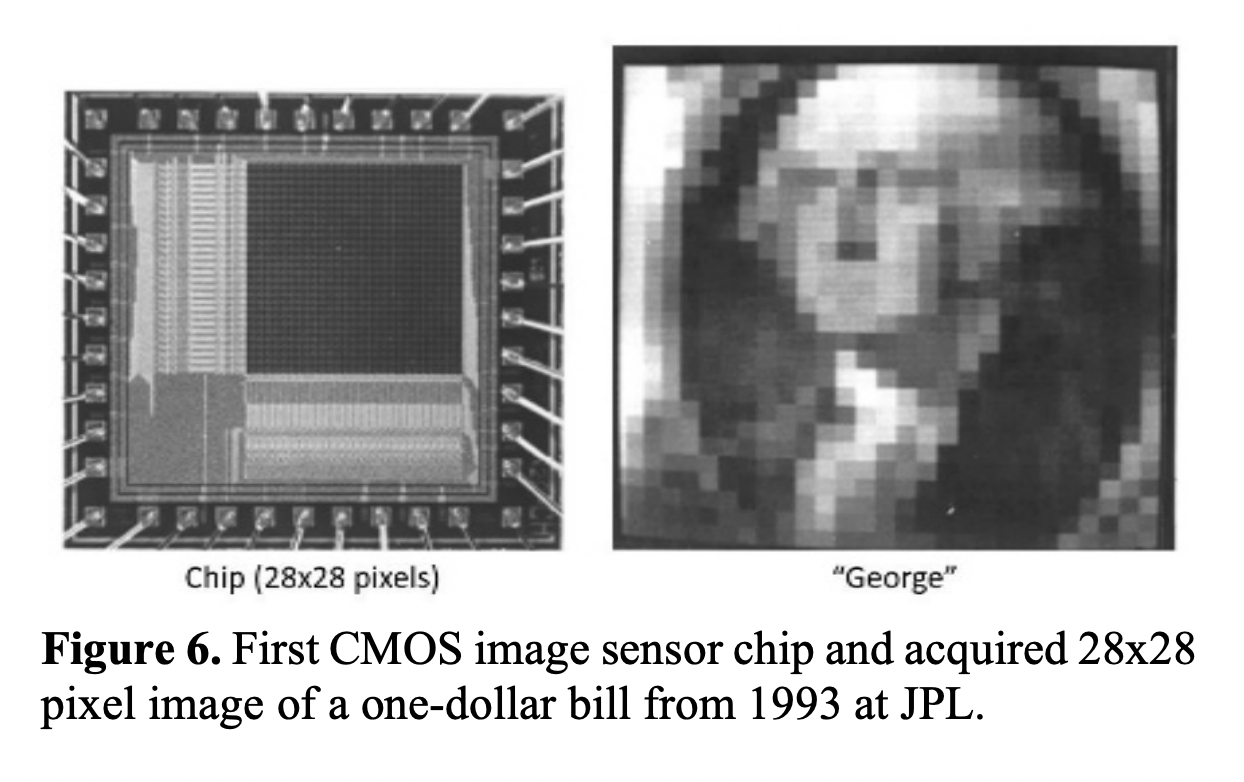
\includegraphics[width=1\textwidth]{figure01}
    \caption{第一个CMOS感光元件和其拍摄的照片(照片为1美元钞票上的华盛顿像)}
    \label{F-01}
\end{figure}

\bibstyle{unsrt}
\bibliography{references}{}
\end{document}
